\chapter{Bridge模式}
\section{Bridge模式的概念}
\subsection{Bridge定义}
桥接(Bridge)模式的定义如下:将抽象与实现分离,使它们可以独立变化。它是用组合关系代替继承关系来实现,从而降低了抽象和实现这两个可变维度的耦合度。
\subsection{类的层次结构}
\begin{itemize}
	\item 类的功能层次结构
	\item 类的实现层次结构
\end{itemize}
类的层次结构两个作用:
\begin{enumerate}
	\item 希望增加新功能时:父类具有基本功能,在子类中增加新的功能;
	\item 希望增加新的实现时:父类通过声明抽象方法来定义接口,子类通过实现来实现接口。
\end{enumerate}
这两个层次分离为两个独立的类的层次结构,如果只是简单分开,两者之间必然缺少联系,
所以需要增加Bridge。
\subsection{优点}
\begin{enumerate}
	\item 由于抽象与实现分离,所以扩展能力强;
	\item 其实现细节对客户透明。
\end{enumerate}
\subsection{缺点}
由于聚合关系建立在抽象层,要求开发者针对抽象化进行设计与编程,这增加了系统的理解与设计难度。
\subsection{应用场景}
\begin{enumerate}
	\item 当一个类存在两个独立变化的维度,且这两个维度都需要进行扩展时。
	\item 当一个系统不希望使用继承或因为多层次继承导致系统类的个数急剧增加时。
	\item 当一个系统需要在构件的抽象化角色和具体化角色之间增加更多的灵活性时。
\end{enumerate}
\subsection{模式的角色}
\subsubsection{Abstraction抽象化}
类的功能层次的最上层,使用Implementor实现基本功能,保存了Implementor实例。
\subsubsection{RefinedAbstraction改善后抽象化}
在Abstraction角色上增加新的功能。
\subsubsection{Implementor实现者}
类的实现层次结构的最上层,定义了用于实现Abstraction角色的接口的方法。
\subsubsection{ConcreteImplementor具体实现者}
负责实现在Implementor中定义的接口。
\section{Bridge实现——例一}
\begin{table}[!h]
	\begin{tabular}{|l|l|l|}
		\hline
		在桥的哪一侧&名字&名字\\
		\hline
		类的功能层次结构&Display&负责“显示”的类\\
		\hline
		类的功能层次结构&CountDisplay&增加了“只显示规定类次数”这一功能的类\\
		\hline
		类的实现层次结构&DisplayImpl&负责“显示”的类\\
		\hline
		类的实现层次结构&StringDisplayImpl&“用字符串显示”的类\\
		\hline
	\end{tabular}
\end{table}
\begin{lstlisting}
public class Display {
	private DisplayImpl impl;
	public Display(DisplayImpl impl) {
		this.impl = impl;
	}
	public void open() {
		impl.rawOpen();
	}
	public void print() {
		impl.rawPrint();
	}
	public void close() {
		impl.rawClose();
	}
	public final void display() {
		open();
		print();
		close();
	}
}
\end{lstlisting}
\begin{lstlisting}
public class CountDisplay extends Display {
	public CountDisplay(DisplayImpl impl) {
		super(impl);
	}
	public void multiDisplay(int times) {
		open();
		for (int i = 0; i < times; i++) {
			print();
		}
		close();
	}
}
\end{lstlisting}
\begin{lstlisting}
public abstract class DisplayImpl {
	public abstract void rawOpen();
	public abstract void rawPrint();
	public abstract void rawClose();
}
\end{lstlisting}
\begin{lstlisting}
public class StringDisplayImpl extends DisplayImpl {
	private String string;
	private int width;
	public StringDisplayImpl(String string) {
		this.string = string;
		this.width = string.getBytes().length;
	}
	public void rawOpen() {
		printLine();
	}
	public void rawPrint() {
		System.out.println("|" + string + "|");
	}
	public void rawClose() {
		printLine();
	}
	public void printLine() {
		System.out.print("+");
		for (int i = 0; i < width; i++) {
			System.out.print("-");
		}
		System.out.println("+");
	}
}
\end{lstlisting}
\begin{lstlisting}
public class Main {
	public static void main(String[] args) {
		Display d1 = new Display(new StringDisplayImpl("Hello, China."));
		Display d2 = new CountDisplay(new StringDisplayImpl("Hello, World."));
		CountDisplay d3 = new CountDisplay(new StringDisplayImpl("Hello, Universe."));
		d1.display();
		d2.display();
		d3.display();
		d3.multiDisplay(5);
	}
}
\end{lstlisting}
\section{Bridge实现——例二}
\begin{figure}[!h]
	\centering
	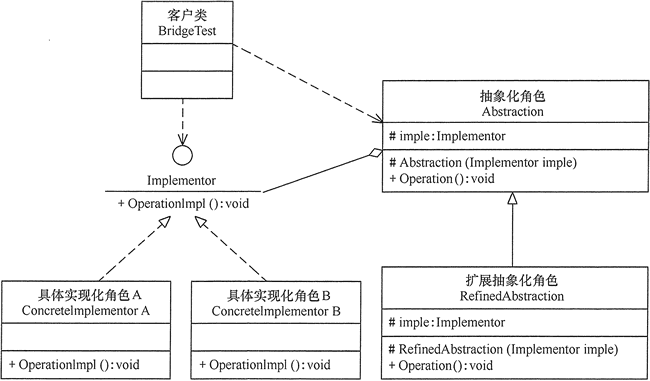
\includegraphics[width=0.8\textwidth]{image/9-1}
	\caption{Bridge实现的类图}
\end{figure}
\begin{lstlisting}
//实现化角色
interface Implementor {
	public void OperationImpl();
}

//具体实现化角色
class ConcreteImplementorA implements Implementor {
	public void OperationImpl() {
		System.out.println("具体实现化(Concrete Implementor)角色被访问");
	}
}
\end{lstlisting}
\begin{lstlisting}
abstract class Abstraction {
	protected Implementor imple;
	protected Abstraction(Implementor imple) {
		this.imple = imple;
	}
	public abstract void Operation();
}

//扩展抽象化角色
class RefinedAbstraction extends Abstraction {
	protected RefinedAbstraction(Implementor imple) {
		super(imple);
	}
	public void Operation() {
		System.out.println("扩展抽象化(Refined Abstraction)角色被访问");
		imple.OperationImpl();
	}
}
\end{lstlisting}
\begin{lstlisting}
public class BridgeTest {
	public static void main(String[] args) {
		Implementor imple = new ConcreteImplementorA();
		Abstraction abs = new RefinedAbstraction(imple);
		abs.Operation();
	}
}
\end{lstlisting}
\section{Bridge模式的扩展}
有时桥接(Bridge)模式可与适配器模式联合使用。当桥接(Bridge)模式的实现化角色的接口与现有类的接口不一致时,可以在二者中间定义一个适配器将二者连接起来
\begin{figure}
	\centering
	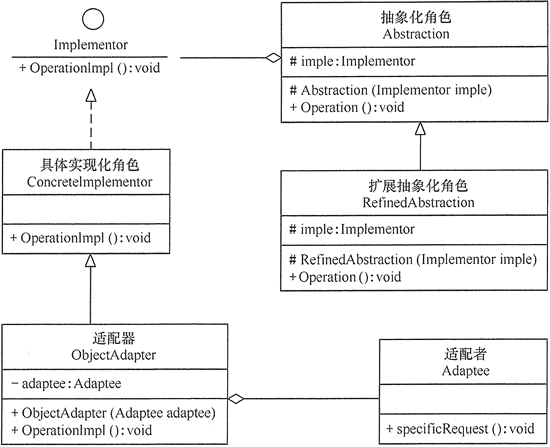
\includegraphics[width=0.8\textwidth]{image/9-2}
	\caption{桥接模式的扩展}
\end{figure}
\section{扩展思路}
\begin{enumerate}
	\item 桥接模式将功能和实现分开,有利于对它们进行扩展,如在不同OS运行,类的实现层次可以表现为OS依赖的部分。
	\item 继承是强关联,委托是弱关联;
\end{enumerate}
\section{相关设计模式}
\begin{enumerate}
	\item Template Method使用了类的实现层次结构,父类调用抽象方法,而子类实现抽象方法;
	\item Abstract Factory为了实现具体实现者角色,有时会使用抽象模工厂模式;
	\item Adapter模式可以为桥接提供功能相似但接口不同的类。
\end{enumerate}